% Document format :
\documentclass[12pt,a4paper]{article}
\usepackage[french]{babel}
\usepackage[a4paper,left=1.5cm,right=1.5cm,top=2.5cm,bottom=2.5cm]{geometry}
\usepackage{multicol}

% Figures :
\usepackage{caption}
\usepackage{subcaption}
\usepackage{graphicx}
\usepackage{float}
\newenvironment{Figure}
{\par\medskip\noindent\minipage{\linewidth}}
{\endminipage\par\medskip}

% Other packages :
\usepackage{indentfirst}
\usepackage{tcolorbox}
\usepackage[hidelinks]{hyperref}

%%%%%%%%%%%%%%%%%%%%%%%%%%%%%%%%%%%%%%%%%%%%%%%%%%%%%%%%%%%%%%%%%%%%%%%%%%%%%%%%%%%%%%%%%%%%%%%%%%%%%%%%%%%%%


\begin{document}

	\title{TP Programmation Orientée Objet -- Rapport}
	\author{Damien \textsc{Garcia} -- Florian \textsc{Echelard}}
	\date{Novembre 2022}
	
	\begin{tcolorbox}
		\maketitle		
	\end{tcolorbox}

	\tableofcontents
	
	\listoffigures
	
	\pagebreak


%%%%%%%%%%%%%%%%%%%%%%%%%%%%%%%%%%%%%%%%%%%%%%%%%%%%%%%%%%%%%%%%%%%%%%%%%%%%%%%%%%%%%%%%%%%%%%%%%%%%%%%%%%%%%


	\begin{multicols}{2} %\setlength{\columnseprule}{0.4pt}
		
		\section{Introduction}

		Le but de ce projet est de fournir un outil de gestion de radiographies pour les médecins au sein d'un centre de santé en s'appuyant sur le paradigme de programmation orienté objet. Pour cela, nous avons commencé par établir les objectifs d'ergonomie et d'accessibilité relatifs à ce logiciel, discuté ensuite de l'implémentation en classes et leur interface relationnelle, puis des éléments utilisés au niveau du code pour élargir et préciser l'application.
		
		\subsection{Objectifs}
		
		L'interface définie par le projet doit permettre à un médecin d'accéder aux radiographies de ses patients, ainsi qu'aux données associées à ces radiographies. Un médecin donné, n'aura accès qu'aux radiographies de ses propres patients, mais pas à celles des autres médecins.\\
				
		Du fait de la séparation des accès aux données, des méthodes de recherches, autorisant ou non l'accès à celles-ci doivent être établies et implémentées. De plus certaines de ces données doivent être protégée par mot de passe, notamment le rapport médical associé aux examens médicaux. Dans un objectif de cohérence générale de l'implémentation, nous avons rapidement opté par implémenter un système de \textit{Login}, c'est-à-dire qu'un utilisateur, avant de pouvoir accéder à quelconque donnée, doit s'identifier sur la base de données ce qui permettra par la suite de lui rendre disponible uniquement les dossiers médicaux lui étant associés. \\
		
		\subsection{Approches}
		
		Notre première approche pour gérer les données utilisateurs séparément était de regrouper les éléments d'intérêt dans un classe à l'interface des utilisateurs et de la base de données pour distribuer de manière contrôlée les attributs. Nous avons cependant fait évolué cette idée par la suite pour inclure l'interface et la gestion de la base de donnée dans deux objets séparés, respectivement pour gérer la sauvegarde des données et l'autre pour faire appel aux éléments utilisateurs lors d'une session. \\
				
		Pour la mise en place de la sauvegarde des instances, nous avons envisagé la méthode de \textit{serializing}, qui permet de concevoir l'application en deux états, active et inactive. A l'activation, les données sont téléchargées (\textit{download}), c'est-à-dire que les différents objets sont instanciés, et à la sortie du logiciel sauvegardées (\textit{update}) en format binaire. Le temps qui nous a été alloué pour ce projet, ne nous a pas permis de mettre en place cette méthode, nous avons donc préféré un format texte classique, avec une grammaire bien définie permettant la lecture et l'écriture des instances de manière automatisée.\\
				
		L'interface visuel (= le \og menu\fg{}) ayant accès aux méthodes de la base de données (détaillé par la suite), l'existence d'une classe faisant le lien entre utilisateur et radiographie n'est plus nécessaire. Ces instances sont regroupées dans la \textbf{session}.
		
		
%%%%%%%%%%%%%%%%%%%%%%%%%%%%%%%%%%%%%%%%%%%%%%%%%%%%%%%%%%%%%%%%%%%%%%%%%%%%%%%%%%%%%%%%%%%%%%%%%%%%%%%%%%%%%
		

		\section{Implémentation}
				
		La volonté de proposer plusieurs profils pour ouvrir cette application non seulement au corps médical mais aussi aux patients, nous a motivé à créer une classe parent \textbf{User}, qui possède des attributs concernant les renseignements généraux, soit le nom, le prénom, et le mot de passe. Contrairement au cahier des charges indiquant le besoin de protéger par mot de passe uniquement le compte-rendu médical et les clichés associés, nous avons fait le choix de vérifier l'identité des utilisateurs à l'ouverture de l'interface. Ainsi, l'utilisateur lambda ne peut pas non plus accéder à la liste des examens. Si un utilisateur souhaite consulter son dossier, il doit être inscrit dans la base de données, où créer un compte qui pourra le cas échéant être modifié pour ajouter de nouveaux examens médicaux.\\
		
		Un médecin (classe \textbf{Doctor}) possède en attribut une liste de patient qui lui sont attribués. Des méthodes pour ajouter, supprimer des patients de liste lui sont accessible. Via la classe \textbf{DatabaseHandling}, le médecin peut accéder à la liste de radiographies de chacun de ses patients. Cette classe lui permet d'ajouter, supprimer et modifier des radiographies. \\
		
		Les radiographies (classe \textbf{Radiography}), possèdent un identifiant, un type (\textit{xRay, MRI, ultrasound}) un état permettant de savoir si la radiographie à été effectuée où si elle est programmée à une date ultérieure (\textit{done, pending}) ainsi qu'une date. Les méthodes de cette classe permettent d'ajouter de nouveaux clichés (classe \textbf{Snapshot}) ou d'en supprimer, ainsi que les méthodes pour ajouter ou supprimer le compte-rendu médical (classe \textbf{Report}). \\
		
		Un patient utilisant pourra voir sa liste de radiographies, accéder aux clichés et compte-rendu associés via des méthodes d'accès par identifiant, sans pouvoir en modifier le contenu. Dans un cas où la liste de radiographies est importante, où simplement pour faciliter la recherche, une méthode de recherche par date est accessible au patient (comme au docteur). \\
		
		Comme expliqué précédemment, la classe \textbf{DatabaseHandling} contient les méthodes à sauvegarder les informations des instances vers des fichiers texte, pour former une base de données une fois les modifications effectuées dans le programme : ce sont les méthodes d' \og \textit{upload}\fg{}. Inversement, les fonctions de \og \textit{download}\fg{} permettent au moment de l'ouverture du programme, d'instancier tous les patients, docteurs et radiographies déjà présent dans la base de données. \\
		
		Enfin la classe \textbf{CommandLineInterface} offre des menus interactifs, des visualisations de toutes les informations de la base de données, les options disponibles aux utilisateurs selon leur type (\textbf{Doctor} ou \textbf{Patient}) et envoie par \og message\fg{} les modifications effectuées dans la \og session\fg{} vers \textbf{DatabaseHandling} pour les stocker. \\
		
	\end{multicols}

	\begin{figure}[H]
		\centering
		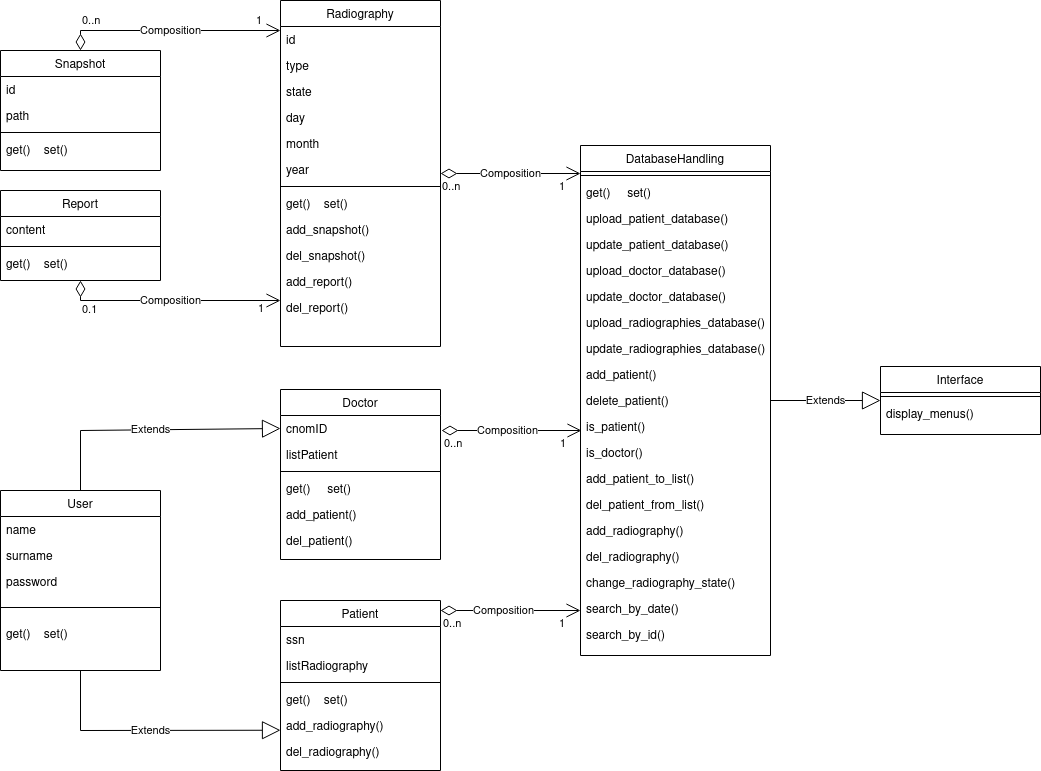
\includegraphics[width=0.8\linewidth]{images/UML_OOP.png}
		\captionof{figure}{Diagramme UML présentant la structure de l'implémentation}
		\label{fig:UML}
	\end{figure}

	\pagebreak


%%%%%%%%%%%%%%%%%%%%%%%%%%%%%%%%%%%%%%%%%%%%%%%%%%%%%%%%%%%%%%%%%%%%%%%%%%%%%%%%%%%%%%%%%%%%%%%%%%%%%%%%%%%%%


	\begin{multicols}{2}
		
		\section{Le logiciel}
		
		\subsection{Description de l'interface}
		
		Nous avons généré un jeux de données composé de patients, médecins et radiographies fictives afin de présenter l'interface.\\
		
		Pour commencer, voici comment le menu principal se présente au lancement de l'application (Fig. \ref{fig:main_menu}) \\
		
		\begin{Figure}
			\centering
			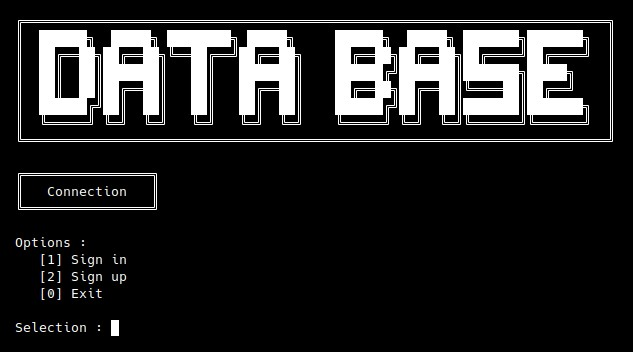
\includegraphics[width=\linewidth]{images/walkthrough/entree.jpg}
			\captionof{figure}{Menu principal}
			\label{fig:main_menu}
		\end{Figure}
		
		Si l'on choisit de se connecter, un formulaire est affiché et donne 3 tentatives d'authentification avant de revenir au menu principal (Fig. \ref{fig:sign_in}). \\
		
		\begin{Figure}
			\centering
			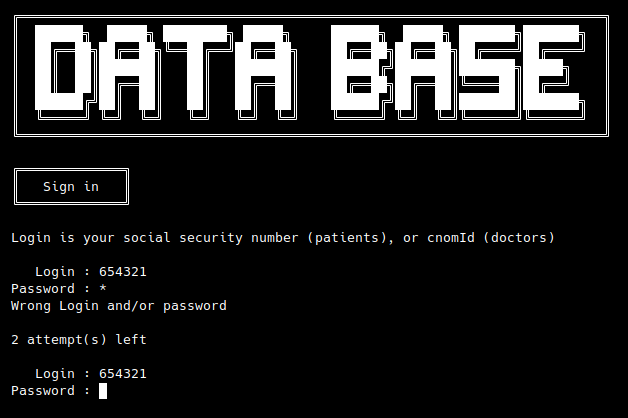
\includegraphics[width=\linewidth]{images/walkthrough/sign_in.png}
			\captionof{figure}{Page de connexion}
			\label{fig:sign_in}
		\end{Figure}
		
		Ici, nous fournissons l'information d'un docteur, il est reconnu dans la base de données et nous pouvons accéder à sa liste de patients, en ajouter et supprimer, ainsi qu'accéder aux données spécifique de chacun des patients de la liste (Fig. \ref{fig:doctor_menu}). \\
		
		\begin{Figure}
			\centering
			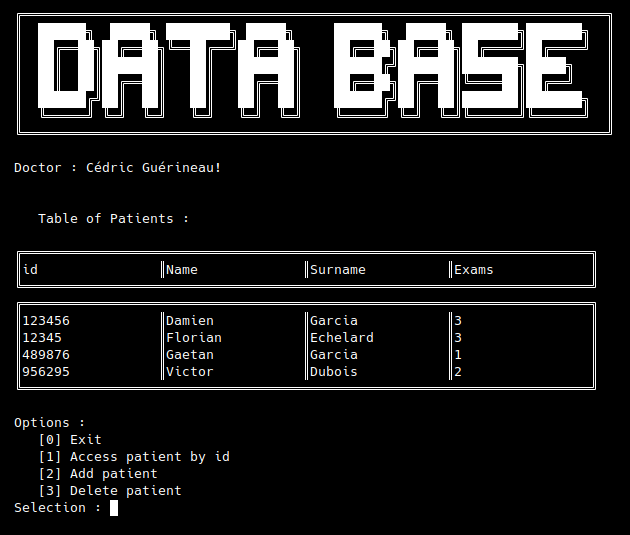
\includegraphics[width=\linewidth]{images/walkthrough/doctor_main.png}
			\captionof{figure}{Liste de patients du menu Docteur}
			\label{fig:doctor_menu}
		\end{Figure}
		
		Si l'on décide d'accéder à un patient grâce à son identifiant, un nouveau menu s'affiche avec la liste des radiographies que cet individu a effectué. Nous pouvons décider de regarder le contenu d'une consultation, que ce soit par un identifiant précis ou la date de consultation, ou encore ajouter et supprimer des consultatations pour ce patient (Fig \ref{fig:patient_menu}). \\
		
		\begin{Figure}
			\centering
			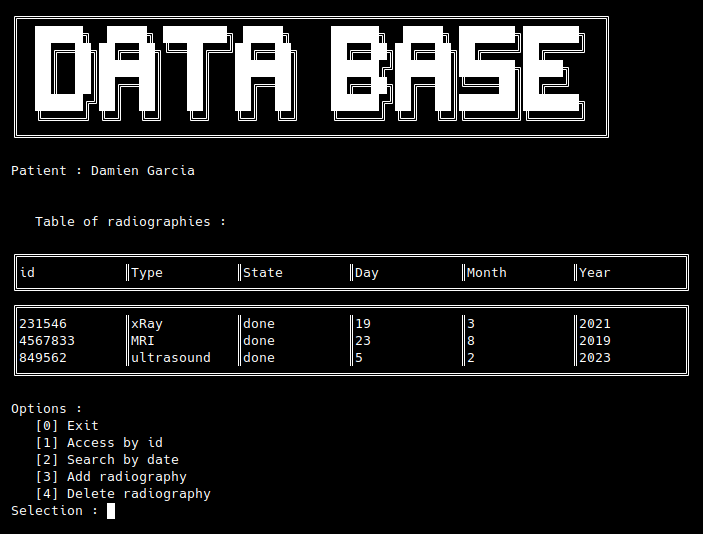
\includegraphics[width=\linewidth]{images/walkthrough/doctor_patient_main.png}
			\captionof{figure}{Le menu spécifique pour un patient}
			\label{fig:patient_menu}
		\end{Figure}
		
		Voici comment de nouvelles radios sont entrées pour un patient (Fig. \ref{fig:add_patient}). \\
		
		\begin{Figure}
			\centering
			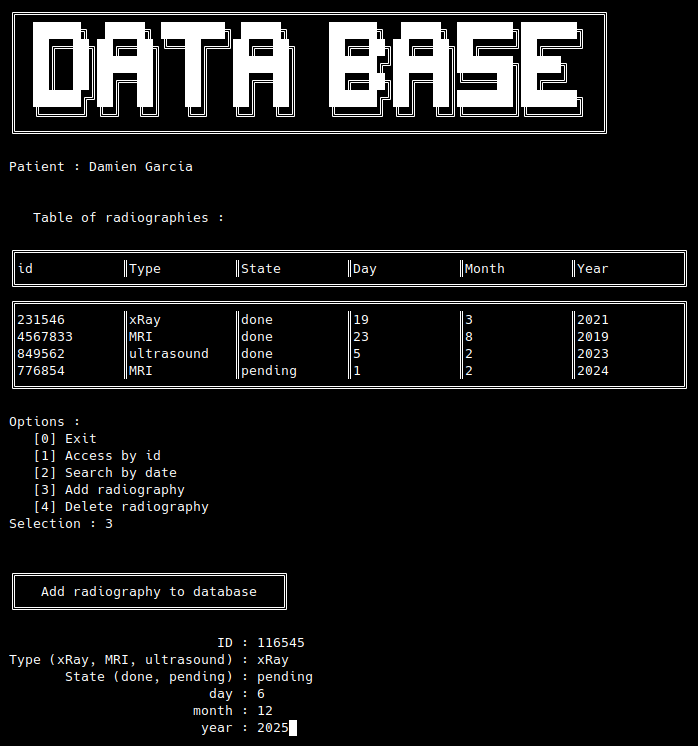
\includegraphics[width=\linewidth]{images/walkthrough/doctor_patient_add.png}
			\captionof{figure}{Ajout de radiographie à un patient}
			\label{fig:add_patient}
		\end{Figure}
		
		Pour retirer une radio, il suffit de donner son identifiant. Si jamais l'identifiant n'existe pas quelque soit la requête, un message d'erreur est retourné (Fig. \ref{fig:err_del_patient}) \\
		
		\begin{Figure}
			\centering
			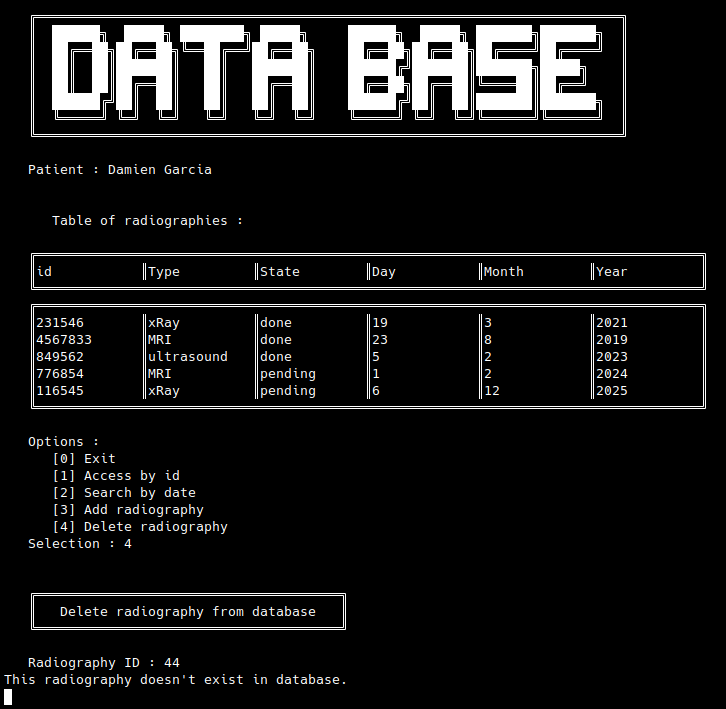
\includegraphics[width=\linewidth]{images/walkthrough/doctor_patient_remove_err.png}
			\captionof{figure}{L'erreur retournée lors de la tentative d'effacement}
			\label{fig:err_del_patient}
		\end{Figure}
		
		L'accès au contenu d'une radiographie permet d'accéder aux clichés et compte-rendu médical associés. Si l'accès se fait via un compte médecin, des options pour éditer le compte-rendu, ajouter et supprimer les clichés sont disponibles (Fig. \ref{fig:search_id}).
		\begin{Figure}
			\centering
			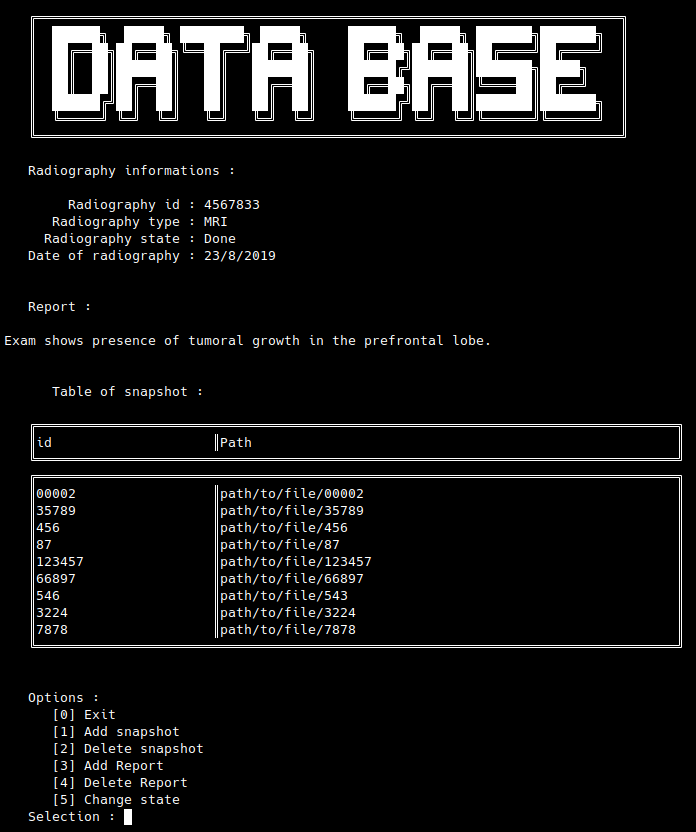
\includegraphics[width=\linewidth]{images/walkthrough/doctor_patient_searchid.png}
			\captionof{figure}{Contenu d'une radiographie pour un patient}
			\label{fig:search_id}
		\end{Figure}
		
		Pour finir, si dans la page de connexion un identifiant de patient est entré, le menu affiché ne sera pas celui d'un docteur, mais une version limitée à la consultation des données, sans options d'édition (Fig. \ref{fig:radio_menu}). \\
		
		\begin{Figure}
			\centering
			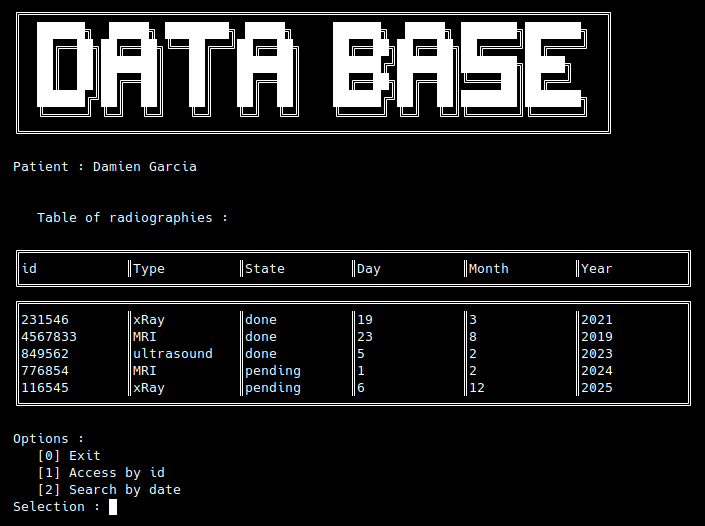
\includegraphics[width=\linewidth]{images/walkthrough/patient_main.png}
			\captionof{figure}{Le menu accessible pour un patient}
			\label{fig:radio_menu}
		\end{Figure}
		
		Dès la fermeture (normale) du programme, toutes les données modifiés dans la session sont sauvegardées et seront disponibles à la prochaine exécution du programme. \\
		
		\begin{tcolorbox}
		\subsection{Notice Utilisateur}

			Bienvenue sur \textbf{DATABASE}, votre outil d'accès aux radiographies. Si vous êtes docteur, vous avez juste à rentrer votre identifiant ou votre mot de passe. Si vous êtes patient, vous pouvez vous connecter si un identifiant vous a été fourni au préalable, ou vous inscrire de vous-même. \\
			
			Une fois cette étape effectuée, vous pourrez consulter vos patients si vous êtes médecin, ou directement les radiographies que vous avez effectué si vous êtes patient. Suivez les instructions à l'écran et entrez les numéros de choix, puis la touche entrée. \\
			
			Cela vous permettra d'accéder ou modifier à vos souhaits la \textbf{DATABASE}.
		\end{tcolorbox}

				
		\section{Perspectives}
		
		Le cahier des charges nous semble respecté dans l'ensemble. De part les contraintes de temps, nous sommes allé à l'essentiel, favorisant le fonctionnement de l'infrastructure interface - base de données plutôt que l'implémentation d'outils poussés pour gérer certaines des tâches de notre application. \\
		
		Parmi celles dont nous percevons une possibilité d'amélioration est le \textit{serialising}. La base de donnée étant du texte pour l'instant, écrit en dur et actualisé à la sortie de l'application ce qui pourrait pour des questions de sécurité et d'optimisation être modifié. Du \og vrai\fg{} \textit{serialising}, compilant les objets en binaire sur le disque dur, permettrait aussi d'implémenter plus aisément des méthodes évitant le conflit entre utilisateur ayant le même identifiant, ce qui est le cas pour l'instant. \\
		
		Le reste des modifications auxquelles nous avons pensé prennent avantage du langage C++ et de son environnement. Par exemple, la gestion des dates et de types de données connus par des librairies spécifiques apporteraient une modularité supplémentaire quant aux vérifications et fonctions que nous souhaitons faire sur celles-ci. Ensuite, en raison de comment nous avons construit notre interface, nous avons fait de la sur-définition de plusieurs constructeurs, et pourrions utiliser un constructeur prenant avantage du polymorphisme, qui regroupe l'initialisation d'élément en commun pour les constructeurs sur-définis. Certaines des classes liées que nous avons écrite pourraient bénéficier de la construction d'un patron dédié, comme le couple Docteur - Patient, ou Photos - Compte rendu. \\
		
		Aussi, nous avons construit la classe abstraite Utilisateur pour l'héritage, mais aurions pu étendre son utilité en lui fournissant des fonctions virtuelles et bénéficier de méthodes optimisées par la suite. \\
		
		Enfin, il serait bénéfique de séparer un certain nombre de méthodes de \textbf{DatabaseHandling} directement dans les classes \textbf{Patient}, \textbf{Doctor} et \textbf{Radiography}, ce qui aurait nécessité de remanier l'architecture UML du logiciel.
		
		\section{Conclusion}
		
		Notre application permet un accès à une base de données dynamique et la séparation de méthodes de consultation et d'édition selon le statut présent dans celle-ci. \\
		
		L'architecture des classes nous permet d'encapsuler les utilisateurs et les données de radiographie dans une interface grâce à une classe de gestion dédiée. \\
		
		Nous avons réussi à remplir le cahier des charges, ainsi que d'aller plus loin pour se rapprocher d'une application réaliste, même si quelques étapes restent à considérer avant cela, autant du point de vue de l'architecture que des fonctionnalités. \\
		
		Après ce premier projet en programmation orientée objet, nous avons pu tirer les conséquences des décisions que nous avons prit initialement, notamment dans l'architecture UML. Ceci nous amènera certainement à penser les futurs projet orienté objet de manière plus informé. \\
		
		\textit{N.B. : Tout numéro de sécurité sociale où identifiant de l'ordre des médecins présent dans notre base de données est totalement fortuit et ne résulte absolument pas d'une attaque informatique sur les serveurs gouvernementaux.} \\
		
	\end{multicols}

%%%%%%%%%%%%%%%%%%%%%%%%%%%%%%%%%%%%%%%%%%%%%%%%%%%%%%%%%%%%%%%%%%%%%%%%%%%%%%%%%%%%%%%%%%%%%%%%%%%%%%%%%%%%%
	
	\section{Annexes}
	
	\begin{Figure}
		\centering
		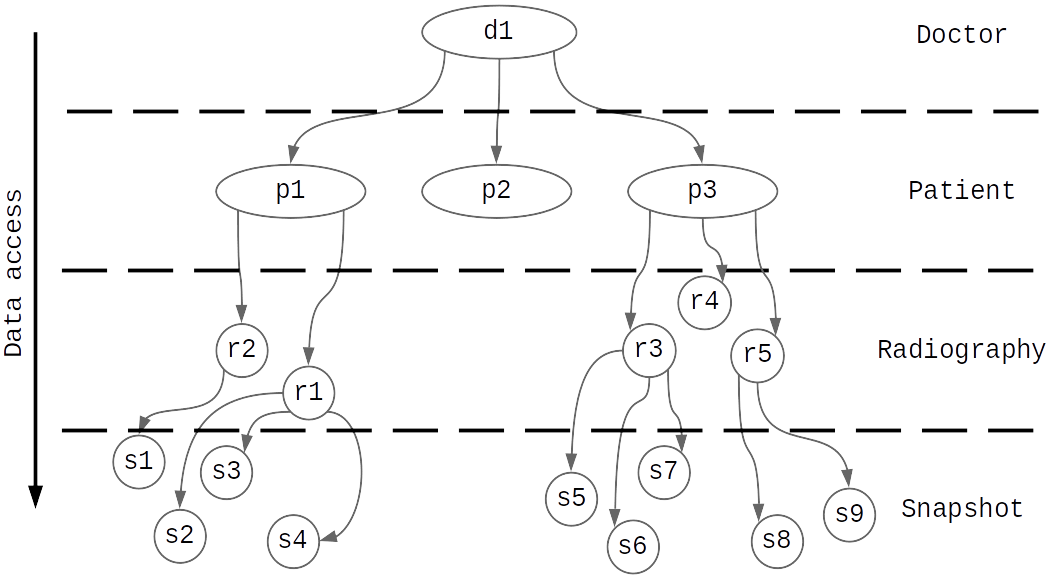
\includegraphics[width=0.7\linewidth]{images/structure.png}
		\captionof{figure}{Structure en \og couches\fg{} de l'outil}
		\subcaption{Dans l'interface, chaque classe présentée sur ce schéma aura accès à toutes les informations des couches inférieures. Par exemple, \textbf{Patient} aura accès à \textbf{Radiography} et \textbf{Snapshot} mais pas à \textbf{Doctor}. Cette notion n'est pas directement représenté dans le diagramme UML mais est induite par les méthodes de l'interface.}
		\label{fig:structure}
	\end{Figure}
	
\end{document}